\chapter{\texorpdfstring{\(SU(5)\)}{SU(5)} 多重態、輕子夸克規範玻色子與質子衰變}

\lectureoverview{標準模型群嵌入 \(SU(5)\) 後，大統一便有了具體形式。為了理解這項陳述的意義，我們先建立所需的表示論基礎：定義表示 \(N\)、其共軛表示 \(\overline N\)、張量積、對稱與反對稱張量，以及伴隨表示。標準模型的一個世代，竟可整合為相當精簡的組合 \(\overline{\mathbf 5}\oplus\mathbf{10}\)。使這種安排如此優美的同一對稱性，也要求存在能使夸克與輕子互相轉換的帶色規範玻色子。這些玻色子的交換使質子衰變成為可能，因而將統一能標推向 \(10^{15}\)--\(10^{16}\,\mathrm{GeV}\)。規範耦合的跑動也指向相近的能標；最後還會談到超對稱，因為納入超對稱後，三種耦合的數值交會會明顯更精確。}

\section{為什麼要從群表示談起？}

大統一理論有許多種提案。我們不逐一綜述，而是拆解其中一個例子，探討三個問題：它為何可行、它要求哪些新粒子，以及實驗在哪些方面對它構成威脅。這個群是 \(SU(5)\)，其關鍵結構特徵是以下嵌入關係
\begin{equation}
SU(3)_c\times SU(2)_L\times U(1)_Y
\subset SU(5).
\label{eq:l10-sm-embedding}
\end{equation}
其中 \(SU(3)_c\) 作用於色，\(SU(2)_L\) 作用於弱同位旋，而 \(U(1)_Y\) 作用於超荷。

超對稱並非這套建構的前提。超對稱與大統一在邏輯上互不蘊含。本講中兩者的關聯在於數值：把超伴子譜納入重整化群計算後，三種規範耦合會更精確地趨近同一個值。

受對稱性作用而彼此互相轉換的粒子，構成該對稱群的一個表示。因此，要分類統一理論中的粒子多重態，得先了解一些表示論。

\subsection{\texorpdfstring{\(SU(2)\)}{SU(2)} 的熟悉例子}

與普通角動量相關的 \(SU(2)\)，和三維空間的旋轉密切相關。更精確地說，\(SU(2)\) 是 \(SO(3)\) 的雙重覆蓋。其不可約表示以
\begin{equation}
j=0,\frac12,1,\frac32,\ldots,
\qquad
\dim(j)=2j+1.
\label{eq:l10-su2-spins}
\end{equation}
為標記。因此，標量是單態，自旋為 \(\tfrac12\) 的粒子是雙重態，自旋為一的粒子是三重態。弱群 \(SU(2)_L\) 是另一種物理對稱性，雖然兩者的抽象群論相同。

\section{定義表示及其共軛表示}

對於 \(SU(N)\)，定義表示的空間由複數 \(N\) 維列向量構成：
\begin{equation}
\psi=
\begin{pmatrix}
\psi_1\\
\psi_2\\
\vdots\\
\psi_N
\end{pmatrix},
\qquad
\psi'_i=U_i{}^j\psi_j,
\qquad
U\in SU(N).
\label{eq:l10-defining}
\end{equation}
它稱為定義表示，也簡稱為 \(\mathbf N\)。矩陣 \(U\) 的大小為 \(N\times N\)，其作用的向量空間維度則為 \(N\)。

複共軛會給出另一個 \(N\) 維表示：
\begin{equation}
\psi_i^*\longmapsto U_i{}^{j*}\psi_j^*,
\label{eq:l10-conjugate}
\end{equation}
此表示記為 \(\overline{\mathbf N}\)。當 \(N>2\) 時，定義表示與共軛表示並不等價。可以互換哪一個稱為粒子表示、哪一個稱為反粒子表示；但一旦選定約定，就必須始終一致。

\begin{classroomqa}
\audiencequestion{\(SU(N)\) 中的 \(N\)，會因 \(N\) 是偶數或奇數而異嗎？它指的是矩陣嗎？\lecturetimestamp{00:07:33}}
\lecturerresponse{這裡沒有偶--奇的限制。\(N\) 是定義矩陣的大小，也是定義表示的維度。\(\mathbf N\) 和 \(\overline{\mathbf N}\) 的維度都相同。}
\end{classroomqa}

反粒子的反粒子就是原來的粒子。因此，互換 \(\mathbf N\) 與 \(\overline{\mathbf N}\) 的名稱，只是改變約定，不會改變物理。

\section{張量積與不可約性}

假設一個物體有 \(N\) 種內部態，另一個物體也可獨立地處於相同數目的內部態。忽略位置、動量、自旋，以及除了 \(SU(N)\) 標記以外的所有量子數，這一對物體共有
\begin{equation}
N\times N=N^2
\label{eq:l10-product-count}
\end{equation}
種態。若第一個物體處於態 \(\psi_i\)，第二個處於態 \(\phi_j\)，兩者的乘積可寫成
\begin{equation}
\Psi_{ij}=\psi_i\phi_j,
\qquad
\Psi'_{ij}=U_i{}^kU_j{}^\ell\Psi_{k\ell}.
\label{eq:l10-tensor-transform}
\end{equation}
這就是張量積 \(\mathbf N\otimes\mathbf N\)。

\begin{classroomqa}
\audiencequestion{答案為 \(N^2\)，而不是 \(N^2-1\)，這是為什麼？允許兩個粒子具有相同的內部標記，會違反不相容原理嗎？\lecturetimestamp{00:10:22}}
\lecturerresponse{這裡的兩個位置可以區分：一個物體固定在一處，另一個固定在別處。泡利不相容原理約束的是包含位置在內的完整量子態，不會排除這些 \(N^2\) 種內部標記組合中的任何一種。數目 \(N^2-1\) 則會在稍後的另一種乘積中，因無跡條件而出現。}
\end{classroomqa}

\(N^2\) 維乘積表示通常是可約的。如果一個表示包含某個真子空間，且群的作用會將該子空間映回自身，這個表示便是可約的。可以將這些不變子空間分離出來，視為較小的表示；若不存在這種真子空間，該表示便是不可約的。

\subsection{對稱張量與反對稱張量}

每個二階張量都可唯一分解為
\begin{align}
\Psi_{ij}
&=\Psi^{(S)}_{ij}+\Psi^{(A)}_{ij},\\
\Psi^{(S)}_{ij}
&=\frac12(\Psi_{ij}+\Psi_{ji}),\\
\Psi^{(A)}_{ij}
&=\frac12(\Psi_{ij}-\Psi_{ji}).
\label{eq:l10-sym-anti}
\end{align}
這兩部分分別滿足
\begin{equation}
\Psi^{(S)}_{ij}=\Psi^{(S)}_{ji},
\qquad
\Psi^{(A)}_{ij}=-\Psi^{(A)}_{ji}.
\end{equation}
式~\eqref{eq:l10-tensor-transform}使兩種條件各自保持不變，因此群變換不會將對稱部分與反對稱部分互相混合。

\editorialnote{講義將一般情形的計數留作練習。對稱部分與反對稱部分的維度分別為 \(N(N+1)/2\) 和 \(N(N-1)/2\)，兩者相加為 \(N^2\)。}

\begin{figure}[htbp]
\centering
\includegraphics[width=0.78\textwidth]{lecture_10_figure_02.png}
\lectureframe{00:17:57.500}
\caption{兩個自旋為 \(\tfrac12\) 的態所構成的完整分解：三個對稱態與一個反對稱態。}
\label{fig:l10-spin-decomposition}
\end{figure}

對於 \(SU(2)\) 的定義二重態，
\begin{equation}
\mathbf2\otimes\mathbf2=\mathbf3_S\oplus\mathbf1_A.
\label{eq:l10-two-two}
\end{equation}
若以 \(u\) 和 \(d\) 表示兩個基底態，對稱三重態為
\begin{align}
\ket{1,1}&=\ket{uu},\\
\ket{1,0}&=\frac{1}{\sqrt2}\bigl(\ket{ud}+\ket{du}\bigr),\\
\ket{1,-1}&=\ket{dd},
\end{align}
反對稱單態則為
\begin{equation}
\ket{0,0}
=\frac{1}{\sqrt2}\bigl(\ket{ud}-\ket{du}\bigr).
\end{equation}
這就是熟悉的兩個自旋為 \(\tfrac12\) 的角動量相加：四個原始態重新組合成自旋一態與自旋零態。

\section{粒子與反粒子：伴隨表示}

現在將定義表示與其共軛表示相乘。此乘積仍有 \(N^2\) 個分量，但變換方式如同矩陣：
\begin{equation}
M_i{}^j\in\mathbf N\otimes\overline{\mathbf N},
\qquad
M\longmapsto U M U^\dagger.
\label{eq:l10-matrix-transform}
\end{equation}
這和 \(\mathbf N\otimes\mathbf N\) 不同；一個基本表示指標與一個反基本表示指標之間，沒有有意義的交換對稱性。自然的分解方式是
\begin{equation}
M
=
\frac{\operatorname{tr}M}{N}\,\mathbf1_N
+
\left(M-\frac{\operatorname{tr}M}{N}\,\mathbf1_N\right).
\label{eq:l10-trace-split}
\end{equation}
第一項是單態，無跡部分則是伴隨表示：
\begin{equation}
\mathbf N\otimes\overline{\mathbf N}
=\mathbf1\oplus\mathbf{Adj},
\qquad
\dim\mathbf{Adj}=N^2-1.
\label{eq:l10-adjoint}
\end{equation}

\begin{figure}[htbp]
\centering
\includegraphics[width=0.67\textwidth]{lecture_10_figure_04.png}
\lectureframe{00:23:47.500}
\caption{黑板上的結論：\(\mathbf N\otimes\overline{\mathbf N}\) 的無跡部分由 \(N^2-1\) 個分量構成伴隨表示。}
\label{fig:l10-adjoint}
\end{figure}

對於 \(SU(3)\)，這會得到熟悉的八重態：
\begin{equation}
\mathbf3\otimes\overline{\mathbf3}
=\mathbf8\oplus\mathbf1,
\end{equation}
八個膠子在伴隨表示下變換。對於 \(SU(2)\)，伴隨表示的維度為三，其變換方式如同自旋一態。

\section{標準模型的一個世代}

我們觀測到三個世代，但 \(SU(5)\) 對每個世代分別重複相同的建構，並未解釋為何有三個世代。因此，我們聚焦於第一代。

所有場都以左手 Weyl 場表示。右手費米子則以其左手電荷共軛場表示：
\begin{equation}
u^c_L,\qquad d^c_L,\qquad e^c_L.
\label{eq:l10-left-handed-bookkeeping}
\end{equation}
上標 \(c\) 表示電荷共軛。例如，\(d^c_L\) 是電荷為 \(+\tfrac13\) 的左手反下夸克場。

按照標準的 \(SU(5)\) 記號，十五個左手場中有五個組成
\begin{equation}
\overline{\mathbf5}
=
\begin{pmatrix}
\nu_{eL}\\
e_L\\
d^c_{rL}\\
d^c_{gL}\\
d^c_{bL}
\end{pmatrix}.
\label{eq:l10-fivebar}
\end{equation}
排列方式是先放入弱作用的二維區塊，再接著放入色作用的三維區塊。弱作用變換會混合前兩個分量，色變換則混合最後三個分量；非對角的 \(SU(5)\) 生成元會連結這兩個區塊。

\editorialnote{講義將式~\eqref{eq:l10-fivebar}中的欄向量稱為 \(\mathbf5\)，之後又將反對稱多重態稱為 \(\overline{\mathbf{10}}\)。這是將所有表示整體共軛的約定。我們採用現代標準約定 \(\overline{\mathbf5}\oplus\mathbf{10}\)；將每個表示取共軛，就能得到講義中的標記，而不改變物理內容。}

第一代的完整最小粒子清單為
\begin{equation}
\begin{gathered}
\underbrace{Q_L=(u_L,d_L)}_{6}
\oplus
\underbrace{L_L=(\nu_{eL},e_L)}_{2},\\
\underbrace{u^c_L}_{3}
\oplus
\underbrace{d^c_L}_{3}
\oplus
\underbrace{e^c_L}_{1},\\
6+2+3+3+1=15.
\end{gathered}
\label{eq:l10-fifteen}
\end{equation}
最小標準模型中沒有獨立的 \(\nu^c_L\)，因此無法產生可重整化的中微子質量。中微子振盪顯示這個最小模型並不完整：自然界中的中微子具有微小但非零的質量，因此需要擴充模型。

\begin{classroomqa}
\audiencequestion{費米子質量使左手態轉變為右手態時，也會使粒子變成反粒子嗎？\lecturetimestamp{00:34:00}}
\lecturerresponse{不會。電子質量項會連結左手電子與具有相同電荷的右手電子。在全左手記號中，後者以 \(e^c_L\) 表示，但四分量描述中的粒子仍然是電子。只有中性場才可能具有將粒子與反粒子視為同一者的 Majorana 質量。}
\end{classroomqa}

\section{五重態中可見的規範玻色子}

每個規範對稱性的生成元都對應一個規範場。在式~\eqref{eq:l10-fivebar}中，已可辨認出熟悉的轉換：
\begin{itemize}
\item 弱規範場作用於 \(\nu_{eL}\) 與 \(e_L\) 之間；
\item 膠子作用於 \(d^c_L\) 的三種顏色之間；
\item 中性生成元以對角方式作用；
\item 新的非對角生成元會將輕子分量轉變為帶色分量，或反向轉變。
\end{itemize}

可以將膠子想成攜帶夸克--反夸克的色量子數。講義使用常見的世界線助記法：沿著一條出射反夸克的世界線，從發射頂點往回追蹤，會看到它彷彿是正向運動的夸克。因此，發射出的場攜帶夸克--反夸克對的量子數。以表示論來說，這正是 \(\mathbf3\otimes\overline{\mathbf3}\) 的無跡部分。

對於 \(SU(5)\)，
\begin{equation}
\dim\mathbf{Adj}_{SU(5)}=5^2-1=24.
\end{equation}
這些規範場在標準模型子群下的分解為
\begin{equation}
\mathbf{24}
=
(\mathbf8,\mathbf1)_0
\oplus(\mathbf1,\mathbf3)_0
\oplus(\mathbf1,\mathbf1)_0
\oplus(\mathbf3,\mathbf2)_{-5/6}
\oplus(\overline{\mathbf3},\mathbf2)_{5/6},
\label{eq:l10-adjoint-sm}
\end{equation}
其中有序對表示 \(SU(3)_c\times SU(2)_L\)，下標表示超荷。

\editorialnote{式~\eqref{eq:l10-adjoint-sm}明確呈現講義所畫的區塊結構。前三項包含熟悉的色與電弱規範場；最後兩項包含十二個實自由度，慣稱為 \(X\) 與 \(Y\) 玻色子。}

\begin{figure}[htbp]
\centering
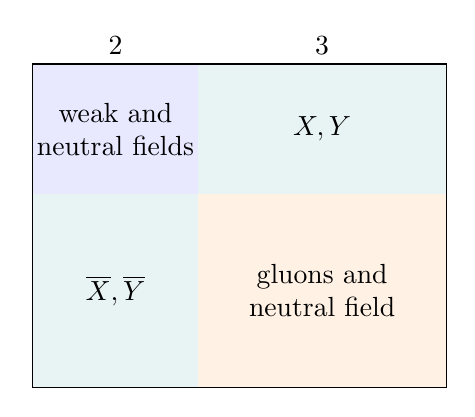
\begin{tikzpicture}[x=1.05cm,y=0.82cm]
  \draw[thick] (0,0) rectangle (5,5);
  \draw[thick] (2,0) -- (2,5);
  \draw[thick] (0,3) -- (5,3);
  \fill[blue!9] (0,3) rectangle (2,5);
  \fill[orange!10] (2,0) rectangle (5,3);
  \fill[teal!9] (2,3) rectangle (5,5);
  \fill[teal!9] (0,0) rectangle (2,3);
  \node[align=center] at (1,4) {weak and\\neutral fields};
  \node[align=center] at (3.5,1.5) {gluons and\\neutral field};
  \node[align=center] at (3.5,4) {\(X,Y\)};
  \node[align=center] at (1,1.5) {\(\overline X,\overline Y\)};
  \node[above] at (1,5) {\(2\)};
  \node[above] at (3.5,5) {\(3\)};
\end{tikzpicture}
\caption{\(SU(5)\)規範場的 \(2\oplus3\) 區塊結構。非對角區塊連結輕子與帶色場。}
\label{fig:l10-gauge-blocks}
\end{figure}

依據 \(Q=T_3+Y\)，式~\eqref{eq:l10-adjoint-sm}中的帶色弱二重態電荷為 \(-\tfrac13\) 和 \(-\tfrac43\)；其共軛態的電荷則為 \(+\tfrac13\) 和 \(+\tfrac43\)。講義將這些粒子稱為 \(X\) 和 \(Y\)，但明確表示不指定哪個名稱對應哪個電荷。物理上不變的是轉換過程與電荷。

\begin{classroomqa}
\audiencequestion{每種新的 \(X\) 或 \(Y\) 規範玻色子都有三種嗎？\lecturetimestamp{00:41:28}}
\lecturerresponse{是的。轉換會連結帶色夸克與無色輕子，因此交換的玻色子必須攜帶兩者之間缺少的色荷。\(X/Y\) 場形成色三重態，能發射或吸收膠子。}
\end{classroomqa}

帶色粒子不會以孤立的漸近態被觀測到。和夸克一樣，新的規範玻色子必須衰變或經歷強子化，形成色中性的組合。

\section{為什麼多重態中包含反下夸克}

\(SU(N)\)的生成元是無跡厄米矩陣。要看出這與「特殊」一詞的關聯，可將無窮小群元素寫為
\begin{equation}
U(\epsilon)=e^{i\epsilon T}.
\end{equation}
么正性給出 \(T^\dagger=T\)，而
\begin{equation}
1=\det U=e^{i\epsilon\operatorname{tr}T}
\end{equation}
對任意的 \(\epsilon\)，則可得
\begin{equation}
\operatorname{tr}T=0.
\label{eq:l10-traceless-generator}
\end{equation}

電荷是生成元的線性組合。在式~\eqref{eq:l10-fivebar}所示的物質欄向量上，它作用為
\begin{equation}
Q_{\overline5}
=
\operatorname{diag}
\left(0,-1,\frac13,\frac13,\frac13\right),
\qquad
\operatorname{tr}Q_{\overline5}=0.
\label{eq:l10-charge-fivebar}
\end{equation}
因此
\begin{equation}
0-1+3\left(\frac13\right)=0.
\end{equation}
若將反下夸克場換成下夸克場，則會得到
\begin{equation}
0-1+3\left(-\frac13\right)=-2,
\end{equation}
這不可能是 \(SU(5)\) 生成元的跡。因此，看似奇怪的反下夸克配置是群結構所強制的。

\section{其餘十個費米子}

另外十個場來自一個二階反對稱張量。在標準約定下，它是下式的反對稱部分：
\begin{equation}
\mathbf5\otimes\mathbf5
=\mathbf{15}_S\oplus\mathbf{10}_A.
\label{eq:l10-five-five}
\end{equation}
講義先暫時寫出共軛量子數
\begin{equation}
\chi=
\begin{pmatrix}
\nu^c\\
e^c\\
d_r\\
d_g\\
d_b
\end{pmatrix}.
\label{eq:l10-aux-five}
\end{equation}
再據此建構這個張量。這只是進行表示張量積時計算用的記帳方式，並非宣稱存在另一個由複合粒子構成的實體五重態。

令
\begin{equation}
\Psi^{ij}=-\Psi^{ji},
\qquad
i,j=1,\ldots,5.
\label{eq:l10-antisym-ten}
\end{equation}
所有對角元素皆為零，下三角部分則由上三角部分決定。因此
\begin{equation}
\dim\mathbf{10}
=\binom52
=\frac{5\cdot4}{2}
=10.
\label{eq:l10-ten-count}
\end{equation}

矩陣中每個分量的電荷，是式~\eqref{eq:l10-aux-five}中對應的列電荷與行電荷之和。由此可直接得到弱--弱位置上的 \(e^c\)、弱--色區塊中的下夸克和上夸克，以及色--色區塊中的反上夸克場。

\begin{classroomqa}
\audiencequestion{正電子和下夸克的標記組合後，所得分量應該是 \(X\) 玻色子嗎？\lecturetimestamp{00:53:08}}
\lecturerresponse{不是。此處建構的是費米子表示，而非規範玻色子的伴隨表示。兩者電荷相加為 \(1-\tfrac13=\tfrac23\)，因此該分量具有上夸克的量子數。}
\end{classroomqa}

一種一致的色符號選擇為
\begin{equation}
\Psi^{ij}=
\begin{pmatrix}
0 & e^c & d_r & d_g & d_b\\
-e^c & 0 & u_r & u_g & u_b\\
-d_r & -u_r & 0 & u_b^c & -u_g^c\\
-d_g & -u_g & -u_b^c & 0 & u_r^c\\
-d_b & -u_b & u_g^c & -u_r^c & 0
\end{pmatrix}.
\label{eq:l10-ten-matrix}
\end{equation}
改變場的相位會改變部分式中顯示的正負號，但不會改變表示或粒子內容。

\begin{figure}[htbp]
\centering
\includegraphics[width=0.83\textwidth]{lecture_10_figure_05.png}
\lectureframe{00:59:17.500}
\caption{課堂上確認各分量與色標記後，完整寫出的 \(2\oplus3\) 反對稱物質矩陣。}
\label{fig:l10-ten-board}
\end{figure}

\begin{classroomqa}
\audiencequestion{十維表示一定要寫成矩陣嗎？也可以寫成欄向量嗎？\lecturetimestamp{00:56:24}}
\lecturerresponse{兩種寫法都可以。可以將十個獨立分量列成欄向量，但反對稱的 \(5\times5\) 矩陣更能呈現 \(SU(5)\) 如何作用於兩個指標，因此所含資訊更豐富。}
\end{classroomqa}

\begin{classroomqa}
\audiencequestion{在色--色區塊中，標記為 \(u\) 的分量是否應該是反上夸克場？\lecturetimestamp{00:57:51}}
\lecturerresponse{是。黑板上的標記更正為 \(u^c\)，也就是左手反上夸克場。兩個下型基底態的電荷相加為 \(-\tfrac23\)，正是反上夸克的電荷。}
\end{classroomqa}

\begin{classroomqa}
\audiencequestion{矩陣中的幾個分量沒有標示顏色。它們仍然守恆嗎？\lecturetimestamp{00:58:05}}
\lecturerresponse{是。三個色的位置分別代表紅、綠、藍。省略色標記只是為了讓內容更清楚。}
\end{classroomqa}

兩個色基本表示組成的反對稱組合，會以反色表示變換：
\begin{equation}
\wedge^2\mathbf3\simeq\overline{\mathbf3},
\qquad
(rg,rb,gb)\sim(\overline b,-\overline g,\overline r).
\label{eq:l10-anticolor}
\end{equation}
因此，色--色區塊中的三個獨立分量，恰好構成反上夸克的反色三重態。

現在，一個世代的粒子已整理為
\begin{equation}
\overline{\mathbf5}\oplus\mathbf{10}.
\label{eq:l10-family}
\end{equation}
值得注意的是，\(u_L\) 和 \(u^c_L\) 位於同一個不可約多重態中；但 \(d_L\) 與 \(d^c_L\)，以及 \(e_L\) 與 \(e^c_L\)，則各自位於不同的多重態。

\begin{classroomqa}
\audiencequestion{若規範變換只在各表示內作用，質量怎麼能連結位於五重態共軛表示與十重態中的場？\lecturetimestamp{01:00:40}}
\lecturerresponse{規範玻色子不會將一個不可約物質表示轉換成另一個表示。希格斯場與 Yukawa 耦合則可以連結不同表示，同時形成整體上 \(SU(5)\) 不變的交互作用；希格斯場取得真空期望值後，這些交互作用便會產生質量。}
\end{classroomqa}

\section{規範玻色子如何使分量轉換}

表示建構完成後，便可將規範玻色子的作用理解為使其中的分量彼此轉換。中性玻色子可能不改變標記；弱玻色子使弱位置互換，膠子使色位置互換，而 \(X/Y\) 玻色子則使弱位置與色位置互換。帶電規範玻色子有對應的反粒子，因此每種轉換都有反向過程。

對反對稱張量而言，無窮小變換會作用於任一指標：
\begin{equation}
\delta\Psi^{ij}
=
i\epsilon
\left(
T^i{}_k\Psi^{kj}
+
T^j{}_k\Psi^{ik}
\right).
\label{eq:l10-two-index-action}
\end{equation}
以矩陣來看，第一項使分量沿垂直方向轉換，第二項則沿水平方向轉換。用來建構張量的組成粒子標記只是助記方式；式~\eqref{eq:l10-two-index-action}才是精確的群論陳述。

弱作用的轉換會使 \(d\) 變成 \(u\)，這是中子 {\proseunicodefont β} 衰變在夸克層次的過程。色轉換會改變紅、綠、藍色，但不改變味。非對角轉換則帶來新的過程：
\begin{equation}
\begin{aligned}
d^c&\longleftrightarrow e,
& d^c&\longleftrightarrow\nu,\\
d&\longleftrightarrow u^c,
& u&\longleftrightarrow e^c,
\end{aligned}
\label{eq:l10-leptoquark-shifts}
\end{equation}
其中相應的 \(X/Y\) 場攜帶電荷與色荷的差異。

\begin{classroomqa}
\audiencequestion{第四與第五個位置之間的轉換代表什麼？第一個位置轉到第四個位置又代表什麼？\lecturetimestamp{01:10:36}}
\lecturerresponse{第四--第五個位置之間的轉換會改變顏色，是膠子轉換。第一--第四個位置之間的轉換跨越弱與色區塊，是新的 \(X/Y\) 轉換之一。}
\end{classroomqa}

\begin{classroomqa}
\audiencequestion{可以明確寫出反對稱矩陣下半部的一個分量嗎？\lecturetimestamp{01:11:23}}
\lecturerresponse{可以。下三角的每個分量都是上三角轉置位置分量的負值。寫出其中一個，就能看清這項規則；全部寫出來並不會增加新的態。}
\end{classroomqa}

\section{危險的後果：質子衰變}

\(X/Y\)玻色子可在一個頂點將夸克與輕子耦合，在另一個頂點則與兩個夸克型場耦合。當動量遠小於其質量時，將重玻色子積分消去，會得到形式如下的六維有效交互作用：
\begin{equation}
\mathcal L_{\mathrm{eff}}
\sim
\frac{g_5^2}{M_X^2}\,(qq)(q\ell)
+\text{h.c.}
\label{eq:l10-effective-proton}
\end{equation}
此交互作用分別違反重子數與輕子數守恆，但會保留統一規範交互作用所決定的組合。

黑板上的過程追蹤一個下夸克和一個上夸克經過重玻色子交換。下夸克轉變為正電子，上夸克轉變為反上夸克，另一個上夸克則不參與反應：
\begin{equation}
uud
\longrightarrow
e^++u\overline u.
\label{eq:l10-quark-decay}
\end{equation}
初態是質子。\(u\overline u\)對可經由強子化形成中性 {\proseunicodefont π} 介子，因此得到
\begin{equation}
p\longrightarrow e^++\pi^0.
\label{eq:l10-proton-pion}
\end{equation}

\begin{figure}[htbp]
\centering
\includegraphics[width=0.82\textwidth]{lecture_10_figure_06.png}
\lectureframe{01:16:02.500}
\caption{黑板上完整呈現了質子內部的重玻色子交換過程，並清楚標出旁觀的上夸克與正電子通道。}
\label{fig:l10-proton-board}
\end{figure}

講義也提到 \(p\to e^++\gamma\)，其中夸克--反夸克對透過電磁作用湮滅。相較於直接強子化，此通道會受到額外的電磁抑制。

這種可能性不是模型中可有可無的細節。一旦單群包含連結夸克與輕子的生成元，通常就會預期有違反重子數的過程。如果這些過程發生在一般的弱或電磁作用時間尺度上，原子核、氫以及宏觀物質都無法存續。

\section{質子為何如此長壽？}

\begin{classroomqa}
\audiencequestion{產生 \(X\) 玻色子的耦合，是不是與群中其他部分使用的統一耦合同一個？\lecturetimestamp{01:18:34}}
\lecturerresponse{在統一能標處，是。簡單的 \(SU(5)\) 規範理論只有一個規範耦合 \(g_5\)。統一對稱性破缺後，低能下的強、弱與超荷耦合會以不同方式跑動，因此數值有所不同。}
\end{classroomqa}

若要維持統一結構，就不能把耦合常數任意調得極小。可提供的抑制來自重粒子的傳播子：
\begin{equation}
\mathcal A
\sim
\frac{g_5^2}{M_X^2}.
\label{eq:l10-amplitude}
\end{equation}
振幅平方後會帶來因子 \(g_5^4/M_X^4\)。再結合量綱分析與質子矩陣元素，便可估算衰變率：
\begin{equation}
\Gamma_p
\sim
C_{\mathrm{had}}\,
\frac{\alpha_5^2\,m_p^5}{M_X^4},
\qquad
\alpha_5=\frac{g_5^2}{4\pi},
\label{eq:l10-rate}
\end{equation}
其中 \(C_{\mathrm{had}}\) 包含群因子、重整化效應，以及非微擾強子矩陣元素。

\editorialnote{講義著重於核心的 \(g^4/M_X^4\) 依賴關係，並指出其中省略了質子質量因子。式~\eqref{eq:l10-rate}補回了所需的質量維度，但並未聲稱這是精確的壽命計算。}

\begin{classroomqa}
\audiencequestion{粗略的課堂估計中，因子 \(g^4\) 可能只有 \(10^{-8}\) 左右；這樣就足以使壽命變得夠長嗎？\lecturetimestamp{01:25:13}}
\lecturerresponse{不夠。這個因子確實有所助益，但微觀強作用時間尺度與質子壽命下限之間，相差的數量級遠不止如此。關鍵的抑制必須來自重粒子質量的四次方。}
\end{classroomqa}

若所有質量都在質子質量的量級，自然的時間單位便約為光穿越質子的時間：
\begin{equation}
t_p\sim\frac{1\ \mathrm{fm}}{c}\sim10^{-23}\ \mathrm{s}.
\label{eq:l10-proton-time}
\end{equation}
原初質子的存在本身已顯示其壽命超過宇宙年齡，但實驗室搜尋所給出的限制嚴格得多。講義將這項微觀估計與當時引用的實驗下限
\begin{equation}
\tau_p\gtrsim10^{33}\ \mathrm{yr}.
\label{eq:l10-lifetime-bound}
\end{equation}作比較。

不必觀察單一質子那麼久。若質子壽命為 \(10^{15}\) 年，一個含有 \(10^{15}\) 個質子的樣本，平均每年約會出現一次衰變事件。更一般地，若在時間 \(T\) 內觀察 \(N_p\) 個質子，預期衰變數為
\begin{equation}
\langle n\rangle\simeq\frac{N_pT}{\tau_p}.
\label{eq:l10-event-count}
\end{equation}
含有約 \(10^{33}\) 個質子的探測器只是大型水槽，並非天文尺度的物體：這些質子的總質量約為 \(10^6\) 公斤。觀察這樣的樣本，就能把極長的單一質子壽命轉化為可測量的事件率，或導出更嚴格的壽命下限。

將式~\eqref{eq:l10-rate}與壽命限制結合，可將輕子夸克規範玻色子的質量推至
\begin{equation}
M_X\sim10^{15}\text{--}10^{16}\ \mathrm{GeV},
\label{eq:l10-mx}
\end{equation}
講義以 \(10^{16}\,\mathrm{GeV}\) 作為便於記憶的安全能標。這比普朗克能標低好幾個數量級，因此不會必然與量子場論相矛盾。

\section{\texorpdfstring{\(SU(5)\)}{SU(5)}的對稱性破缺與統一能標}

\(X/Y\)場與標準模型規範場同屬一個 \(SU(5)\) 伴隨多重態。若規範對稱性完全未破缺，就不可能讓部分成員的質量接近 \(10^{16}\,\mathrm{GeV}\)，同時讓光子和膠子保持無質量。因此，對稱性必須自發破缺。

\begin{classroomqa}
\audiencequestion{若 \(SU(5)\) 對稱性未破缺，其所有規範玻色子都會是無質量的嗎？\lecturetimestamp{01:29:37}}
\lecturerresponse{在此處討論的規範理論中，是。規範不變性不允許直接加入共同質量項。希格斯機制可以使與破缺生成元相關的規範玻色子取得質量，同時讓未破缺子群的規範場保持無質量。}
\end{classroomqa}

電弱希格斯機制已展示了這種模式：它使光子與 \(W^\pm\)、\(Z\) 有所區別。大統一則需要另一個高能標序參量，用以區分弱作用的 \(2\) 區塊與色作用的 \(3\) 區塊，並使非對角的 \(X/Y\) 場變得極為沉重。

相較於 \(10^{16}\,\mathrm{GeV}\)，即使質量為 \(100\,\mathrm{GeV}\) 的弱玻色子也微不足道。在遠高於重粒子閾值的能量下，所有規範玻色子的質量都可忽略，完整的 \(SU(5)\) 對稱性便是良好的近似。統一能標的意義就在於此：低能世界並不會明顯呈現 \(SU(5)\) 對稱性；但在足夠高能的過程中，對稱性破缺所造成的質量差異便不再重要。

\section{跑動耦合}

規範耦合隨能量尺度呈對數變化。定義
\begin{equation}
\alpha_i(\mu)=\frac{g_i^2(\mu)}{4\pi},
\end{equation}
其單圈演化形式為
\begin{equation}
\alpha_i^{-1}(\mu)
=
\alpha_i^{-1}(\mu_0)
-\frac{b_i}{2\pi}
\ln\!\left(\frac{\mu}{\mu_0}\right).
\label{eq:l10-running}
\end{equation}
係數 \(b_i\) 取決於規範群，以及所有足以在相關量子迴圈中傳播的粒子。

\editorialnote{若要比較超荷耦合與 \(SU(5)\) 中的非阿貝爾耦合，就必須對 \(g_1\) 採用慣用的大統一正規化。這就是講義提到的數值群論因子來源。}

在實驗室能量下，三種耦合常數的倒數各不相同。按照講座中的定性排序，\(1/\alpha_1\)最大，因為超荷作用最弱；\(1/\alpha_2\)次之；\(1/\alpha_3\)最小，因為強作用最強。無法直接測量不可達能量處的曲線；這些曲線是根據觀測到的低能量值、粒子譜，以及決定貝塔函數的圈圖計算而得。在標準模型的粒子內容下，以\(\log\mu\)為橫軸作圖時，這些曲線幾乎呈直線。

\begin{figure}[htbp]
\centering
\includegraphics[width=0.74\textwidth]{lecture_10_figure_07.png}
\lectureframe{01:36:32.500}
\caption{黑板上的圖顯示，規範耦合常數的倒數在\(10^{16}\,\mathrm{GeV}\)附近逐漸趨近。圈選區域標示出它們並未完全交會。}
\label{fig:l10-running-board}
\end{figure}

在大統一能標以下，對稱性已破缺，輕粒子譜並未構成完整且簡併的\(SU(5)\)多重態，而三個貝塔函數係數也各不相同。因此，耦合常數隨能標演化的速率各異。在高能標處，我們要問的是，它們是否會達到共同的數值：
\begin{equation}
\alpha_1(M_{\mathrm{GUT}})
\stackrel{?}{=}
\alpha_2(M_{\mathrm{GUT}})
\stackrel{?}{=}
\alpha_3(M_{\mathrm{GUT}}).
\label{eq:l10-unification-condition}
\end{equation}

若粒子譜只有非超對稱標準模型中的粒子，這些曲線會在\(10^{15}\)--\(10^{16}\,\mathrm{GeV}\)附近逐漸接近，卻仍有相當大的偏差；講座將吻合程度描述為約百分之十五。值得注意的是，這也恰好是質子穩定性所要求的能標。

\section{最後一個中子問題}

\begin{classroomqa}
\audiencequestion{如果把質子衰變圖中的旁觀上夸克換成下夸克，描述的會是中子衰變嗎？\(X\)玻色子是否會造成影響？\lecturetimestamp{01:36:40}}
\lecturerresponse{這會定義一種大統一理論中的中子衰變道，例如\(n\to e^++\pi^-\)，但那並不是我們熟悉的自由中子衰變。一般的中子貝塔衰變是\(n\to p+e^-+\overline\nu_e\)，由弱作用引起。如果質子--中子的質量排序顛倒，貝塔穩定性也會隨之顛倒；不過，速率慢得多的大統一衰變道仍可能存在。}
\end{classroomqa}

這個區分說明，運動學與新相互作用是兩回事。哪種核子會發生貝塔衰變，取決於質子--中子的質量差；由\(X/Y\)交換造成的重子數破壞，則是另一種受到極大抑制的機制。

\section{超對稱與更廣闊的視野}

加入超對稱夥伴粒子譜會改變式~\eqref{eq:l10-running}中的貝塔函數係數。按照講座的說法，三種外推得到的耦合常數便會以約百分之一的精度交會。這並不能證明超對稱或大統一理論，但這項實證上的吻合，正是人們常將兩者一併討論的原因。

物質多重態還能進一步統一。在
\begin{equation}
SO(10)\supset SU(5),
\end{equation}
之下，一個旋量表示可分解為
\begin{equation}
\mathbf{16}
\longrightarrow
\mathbf{10}\oplus\overline{\mathbf5}\oplus\mathbf1.
\label{eq:l10-so10}
\end{equation}
這個單態自然可認定為左手反中微子，亦即右手中微子的電荷共軛。因此，擴展世代中的全部 16 個場都能納入一個不可約的\(SO(10)\)多重態。

質子衰變實驗持續檢驗這個構想：若未觀測到衰變事件，便提高質子壽命的下限。超對稱大統一模型並不預言單一且普遍適用的質子壽命；額外的重場，以及依賴超對稱夥伴粒子的算符，都可能使主導衰變道與衰變率在很大的範圍內改變。

\editorialnote{在超對稱大統一理論中，色三重態希格斯粒子交換除了能產生本文討論的六維規範玻色子算符，還能產生五維重子數破壞算符。這些算符的係數高度依賴重粒子譜、味結構與超對稱夥伴粒子的質量，這也說明了講座為何提醒我們：單憑超對稱理論，無法推得單一的質子壽命。}

最重要的啟示是其中存在張力，而非已得出定論。群論以驚人的簡潔方式將夸克與輕子納入同一架構；耦合常數隨能標的演化暗示它們可能在高能標匯聚，而超對稱則使這項數值上的暗示更為明確。同一套架構也預言了夸克轉變為輕子的危險過程。因此，任何成功的理論都必須在保有這份優雅的同時，讓質子維持穩定，時間長到幾乎難以想像。呼應講座結尾的祝願：願我們所有的質子都保持穩定。
